\section{Applikationsmodeller}

\subsection{Applikationsmodel for RPi}
\subsubsection{UC1}

\begin{figure}[H]
    \centering
    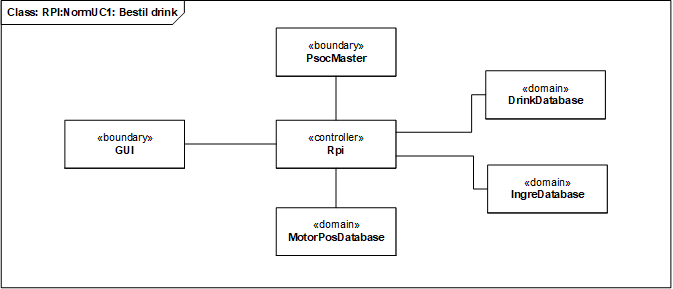
\includegraphics[width=1\textwidth]{Images/Applikationsmodeller/rpi/rpi_klassediagramNormUC1.png}
    \caption{Indledende klassediagram for Rpi i UC1}
    \label{fig:cdUC1Rpi}
\end{figure}

\begin{figure}[H]
    \centering
    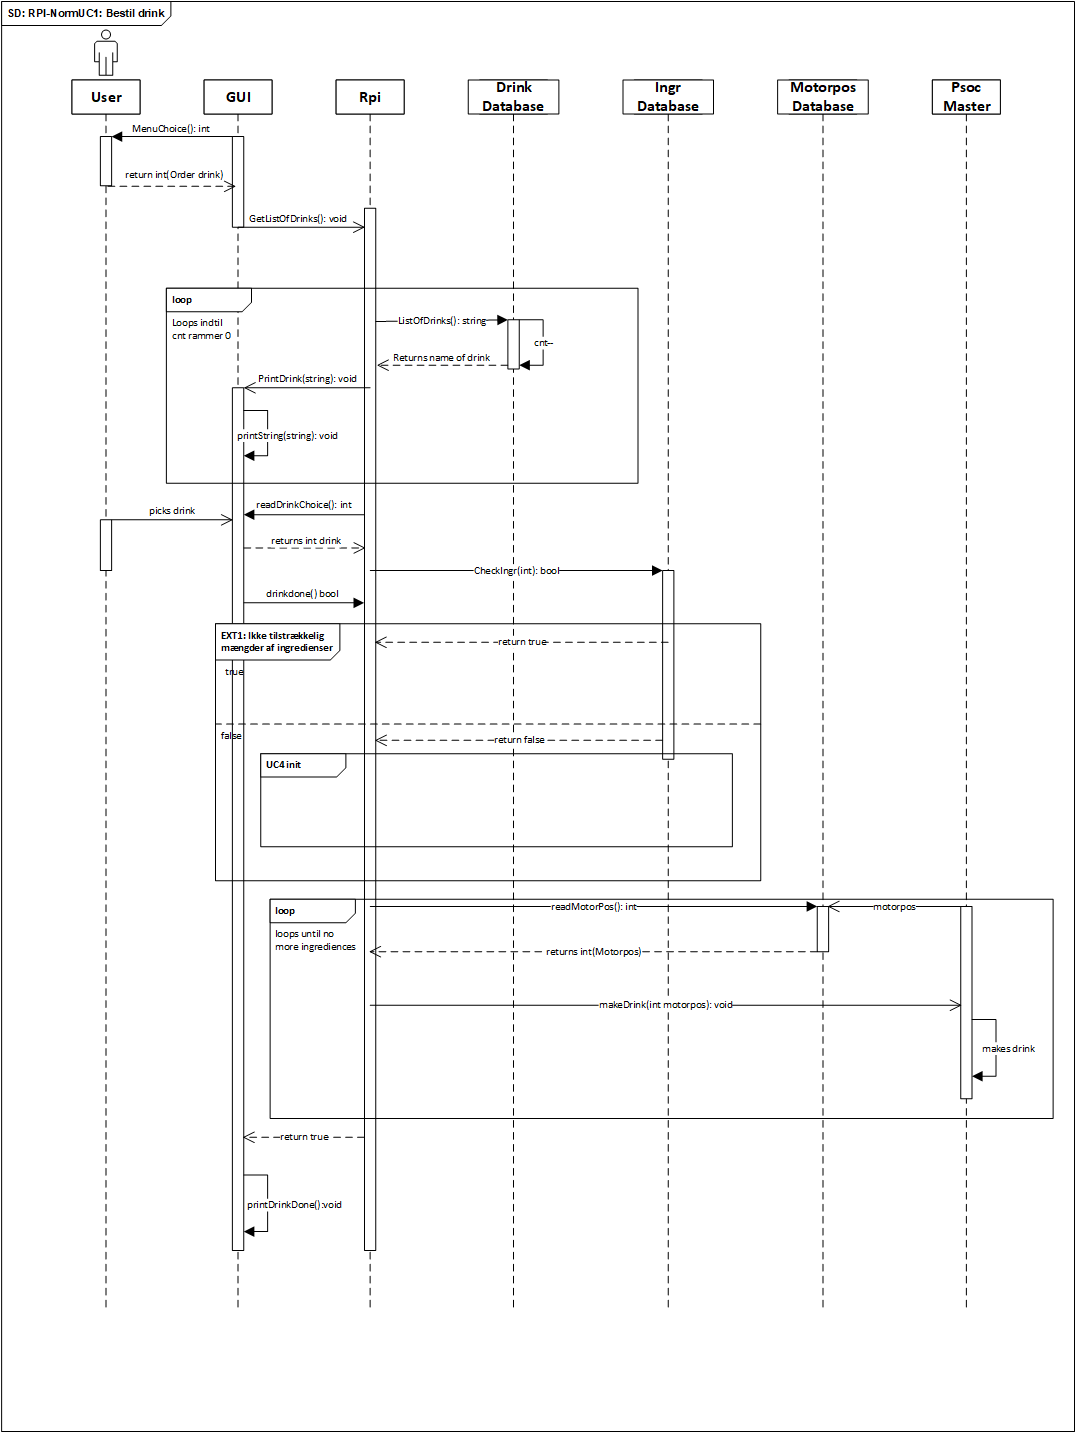
\includegraphics[width=1\textwidth]{Images/Applikationsmodeller/rpi/rpi_sekvensdiagramNormUC1.png}
    \caption{sekvensdiagram for Rpi i UC1}
    \label{fig:sdUC1Rpi}
\end{figure}

\begin{figure}[H]
    \centering
    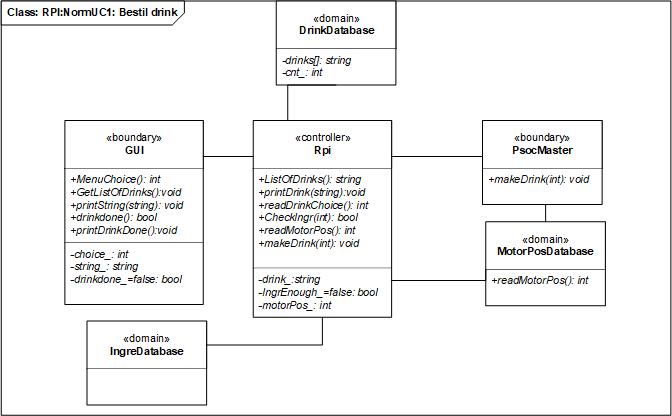
\includegraphics[width=1\textwidth]{Images/Applikationsmodeller/rpi/rpi_UdvidetklassediagramNormUC1.png}
    \caption{Udvidet klassediagram for Rpi i UC1}
    \label{fig:UcdUC1Rpi}
\end{figure}

\subsubsection{UC2}

\begin{figure}[H]
    \centering
    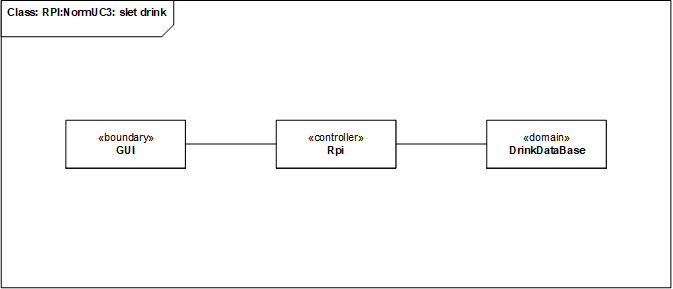
\includegraphics[width=1\textwidth]{Images/Applikationsmodeller/rpi/rpi_klassediagramNormUC3.png}
    \caption{Indledende klassediagram for Rpi i UC2}
    \label{fig:cdUC2Rpi}
\end{figure}

\begin{figure}[H]
    \centering
    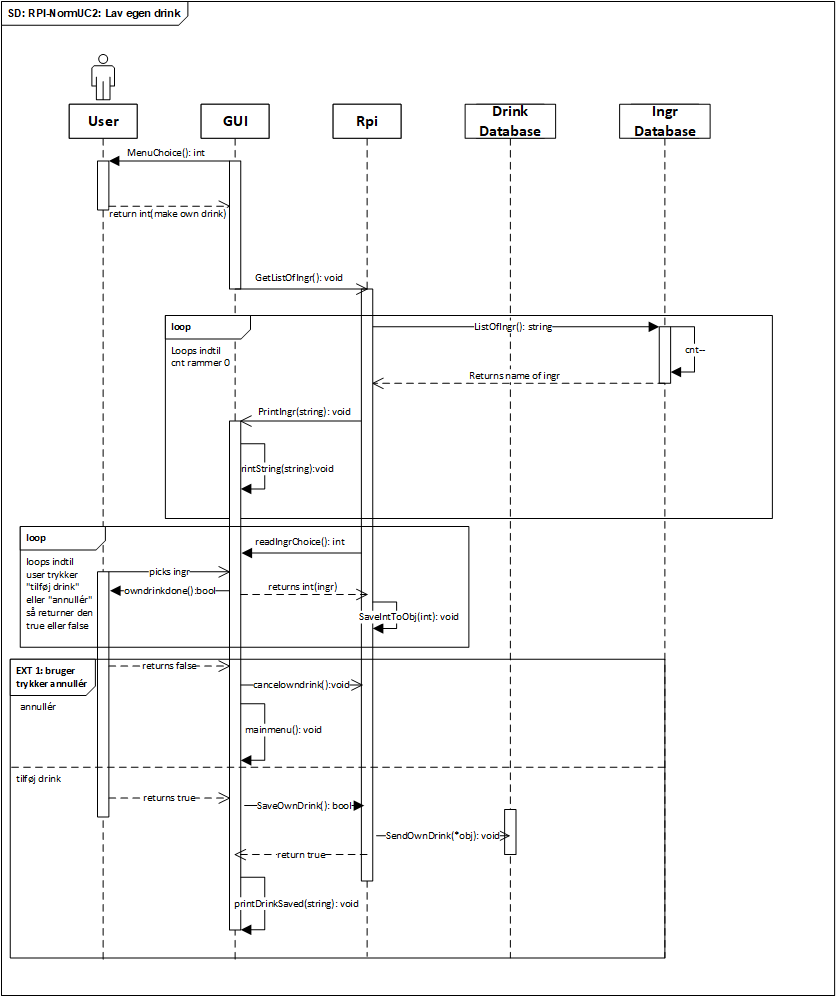
\includegraphics[width=1\textwidth]{Images/Applikationsmodeller/rpi/rpi_sekvensdiagramNormUC2.png}
    \caption{Sekvensdiagram for Rpi i UC2}
    \label{fig:sdUC2Rpi}
\end{figure}

\begin{figure}[H]
    \centering
    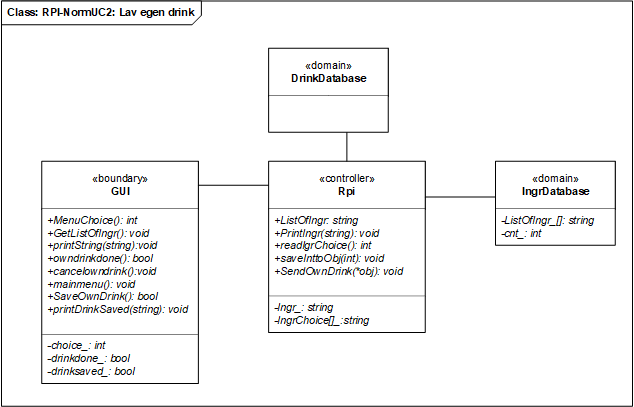
\includegraphics[width=1\textwidth]{Images/Applikationsmodeller/rpi/rpi_UdvidetklassediagramNormUC2.png}
    \caption{Udvidet klassediagram for Rpi i UC2}
    \label{fig:UcdUC2Rpi}
\end{figure}

\subsubsection{UC3}

\begin{figure}[H]
    \centering
    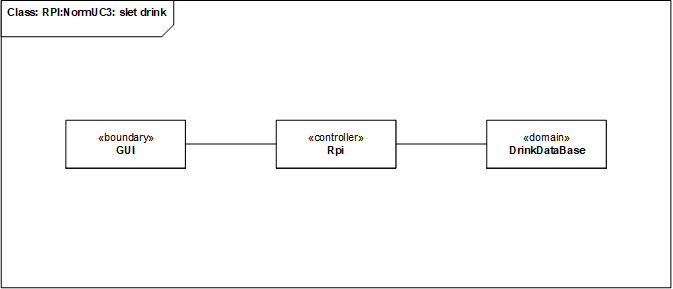
\includegraphics[width=1\textwidth]{Images/Applikationsmodeller/rpi/rpi_klassediagramNormUC3.png}
    \caption{Indledende klassediagram for Rpi i UC3}
    \label{fig:cdUC3Rpi}
\end{figure}

\begin{figure}[H]
    \centering
    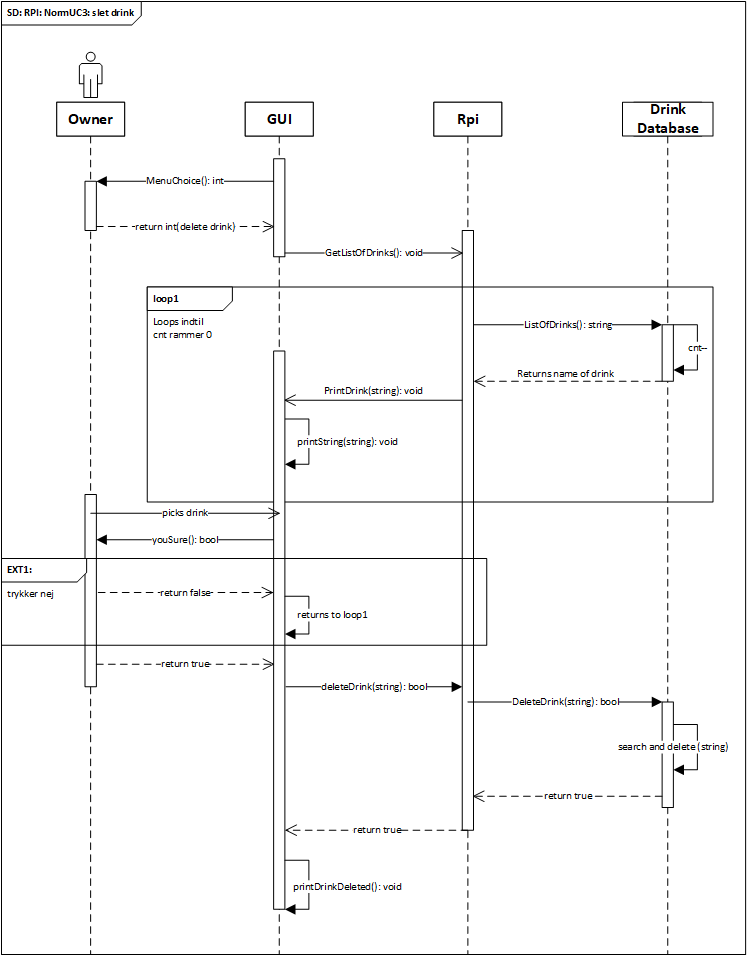
\includegraphics[width=1\textwidth]{Images/Applikationsmodeller/rpi/rpi_sekvensdiagramNormUC3.png}
    \caption{Sekvensdiagram for Rpi i UC3}
    \label{fig:SdUC3Rpi}
\end{figure}

\begin{figure}[H]
    \centering
    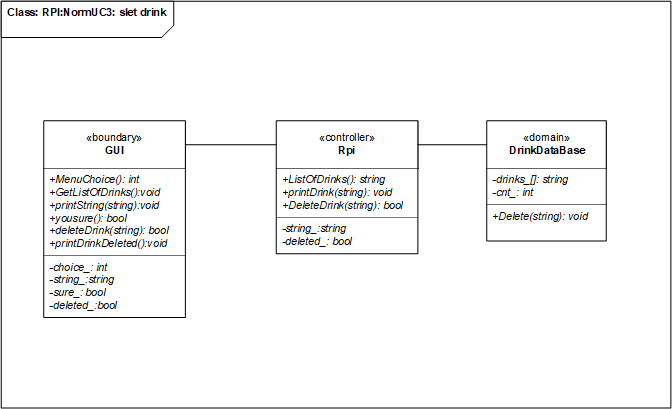
\includegraphics[width=1\textwidth]{Images/Applikationsmodeller/rpi/rpi_UdvidetklassediagramNormUC3.png}
    \caption{Udvidet klassediagram for Rpi i UC3}
    \label{fig:UcdUC3Rpi}
\end{figure}

\subsubsection{UC4}

\begin{figure}[H]
    \centering
    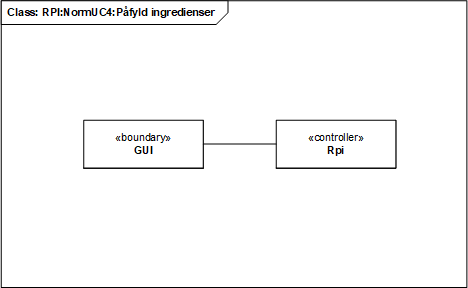
\includegraphics[width=1\textwidth]{Images/Applikationsmodeller/rpi/rpi_klassediagramNormUC4.png}
    \caption{Indledende klassediagram for Rpi i UC4}
    \label{fig:cdUC4Rpi}
\end{figure}

\begin{figure}[H]
    \centering
    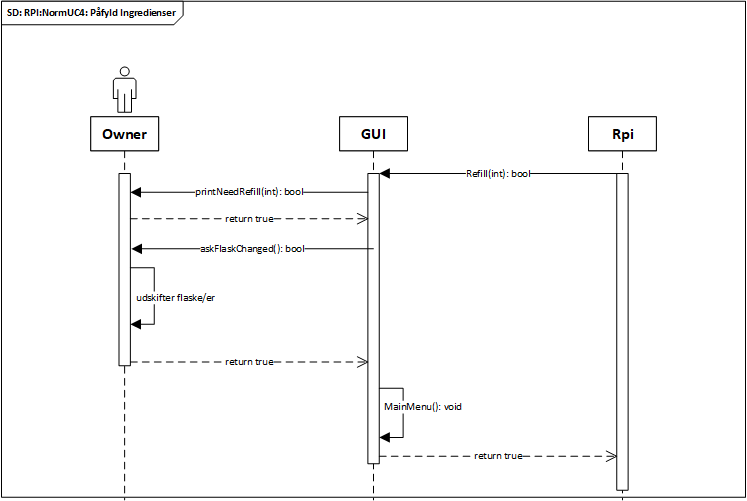
\includegraphics[width=1\textwidth]{Images/Applikationsmodeller/rpi/rpi_sekvensdiagramNormUC4.png}
    \caption{Sekvensdiagram for Rpi i UC4}
    \label{fig:sdUC4Rpi}
\end{figure}

\begin{figure}[H]
    \centering
    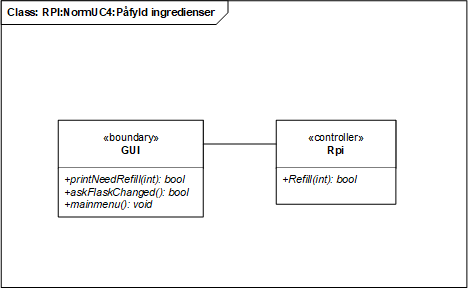
\includegraphics[width=1\textwidth]{Images/Applikationsmodeller/rpi/rpi_UdvidetklassediagramNormUC4.png}
    \caption{Udvidet klassediagram for Rpi i UC4}
    \label{fig:UcdUC4Rpi}
\end{figure}

\subsubsection{UC5}

\begin{figure}[H]
    \centering
    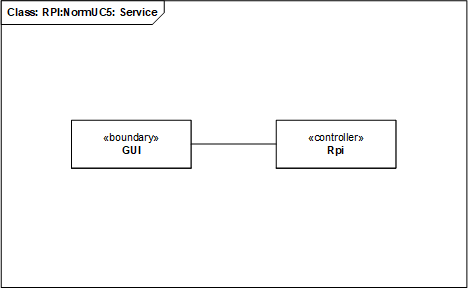
\includegraphics[width=1\textwidth]{Images/Applikationsmodeller/rpi/rpi_klassediagramNormUC5.png}
    \caption{Indledende klassediagram for Rpi i UC5}
    \label{fig:cdUC5Rpi}
\end{figure}

\begin{figure}[H]
    \centering
    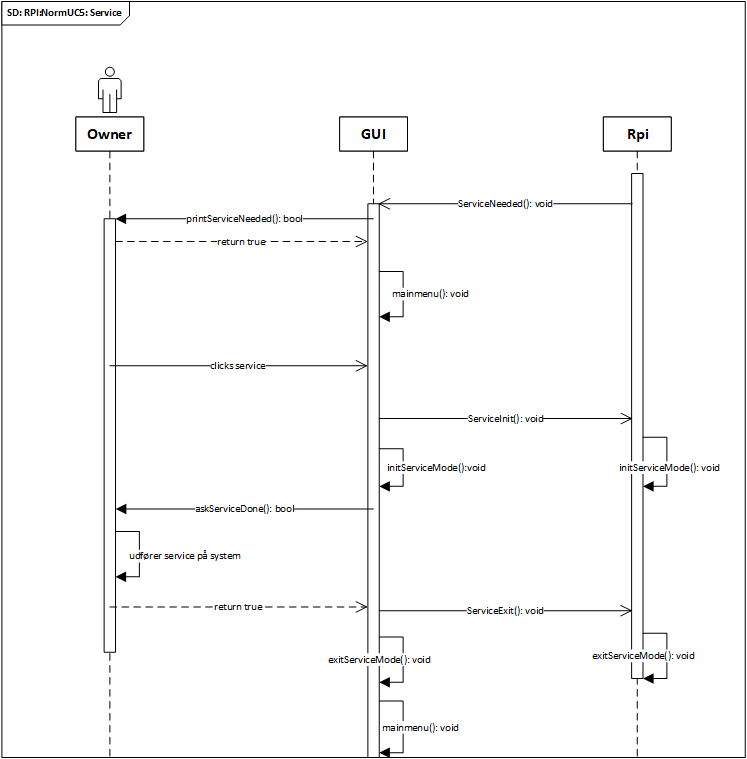
\includegraphics[width=1\textwidth]{Images/Applikationsmodeller/rpi/rpi_sekvensdiagramNormUC5.png}
    \caption{Sekvensdiagram for Rpi i UC5}
    \label{fig:sdUC4Rpi}
\end{figure}

\begin{figure}[H]
    \centering
    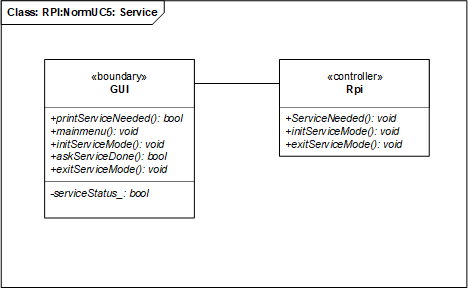
\includegraphics[width=1\textwidth]{Images/Applikationsmodeller/rpi/rpi_UdvidetklassediagramNormUC5.png}
    \caption{Udvidet klassediagram for Rpi i UC5}
    \label{fig:UcdUC5Rpi}
\end{figure}

\subsubsection{TUC1}

\begin{figure}[H]
    \centering
    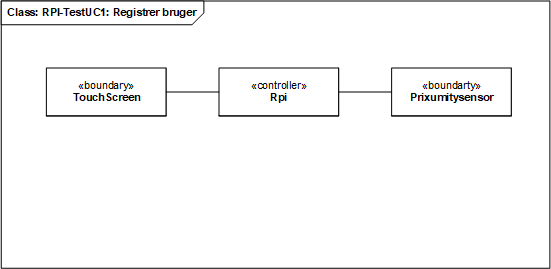
\includegraphics[width=1\textwidth]{Images/Applikationsmodeller/rpi/rpi_klassediagramTestUC1.png}
    \caption{Indledende klassediagram for Rpi i TUC1}
    \label{fig:cdTUC1Rpi}
\end{figure}

\begin{figure}[H]
    \centering
    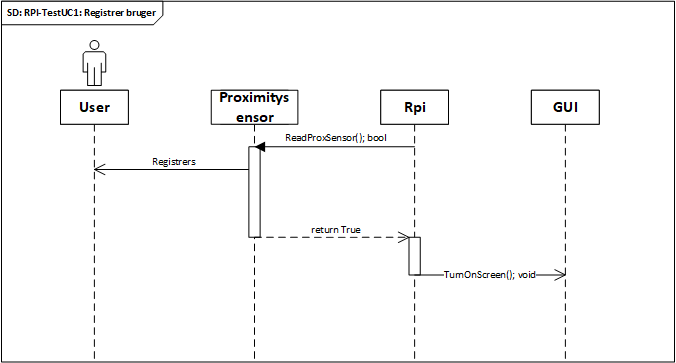
\includegraphics[width=1\textwidth]{Images/Applikationsmodeller/rpi/rpi_sekvensdiagramTestUC1.png}
    \caption{Sekvensdiagram for Rpi i TUC1}
    \label{fig:sdTUC1Rpi}
\end{figure}

\begin{figure}[H]
    \centering
    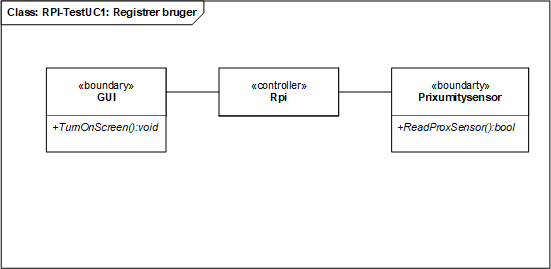
\includegraphics[width=1\textwidth]{Images/Applikationsmodeller/rpi/rpi_UdvidetklassediagramTestUC1.png}
    \caption{Udvidet klassediagram for Rpi i TUC1}
    \label{fig:UcdTUC1Rpi}
\end{figure}

\subsubsection{TUC2}

\begin{figure}[H]
    \centering
    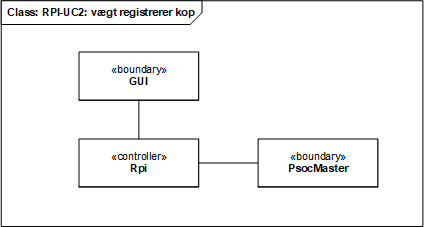
\includegraphics[width=1\textwidth]{Images/Applikationsmodeller/rpi/rpi_klassediagramTestUC2.png}
    \caption{Indledende klassediagram for Rpi i TUC2}
    \label{fig:cdTUC2Rpi}
\end{figure}

\begin{figure}[H]
    \centering
    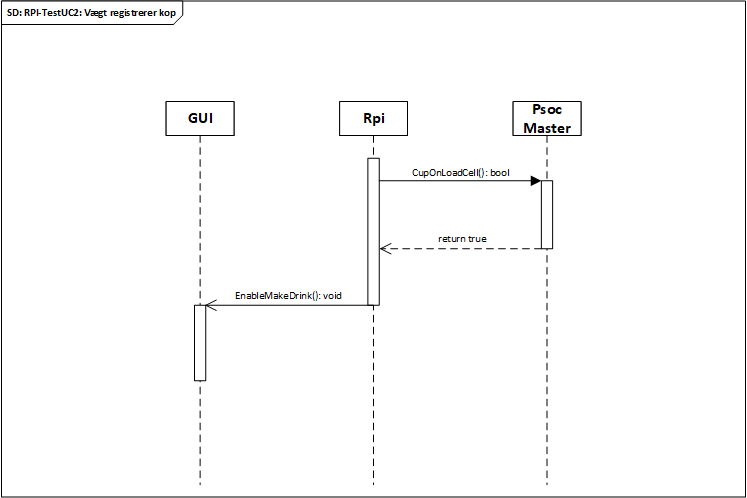
\includegraphics[width=1\textwidth]{Images/Applikationsmodeller/rpi/rpi_sekvensdiagramTestUC2.png}
    \caption{Sekvensdiagram for Rpi i TUC2}
    \label{fig:sdTUC2Rpi}
\end{figure}

\begin{figure}[H]
    \centering
    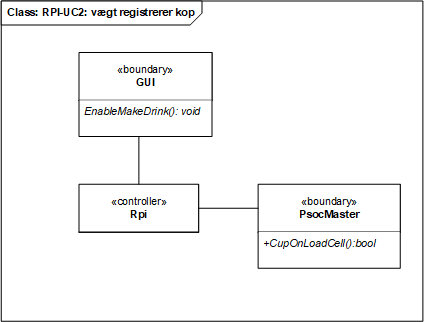
\includegraphics[width=1\textwidth]{Images/Applikationsmodeller/rpi/rpi_UdvidetklassediagramTestUC2.png}
    \caption{Udvidet klassediagram for Rpi i TUC2}
    \label{fig:UcdTUC2Rpi}
\end{figure}

\subsubsection{TUC3}

\begin{figure}[H]
    \centering
    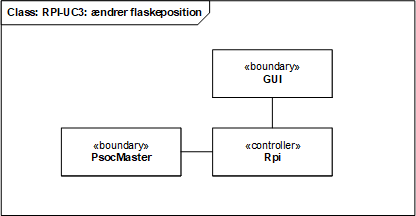
\includegraphics[width=1\textwidth]{Images/Applikationsmodeller/rpi/rpi_klassediagramTestUC3.png}
    \caption{Indledende klassediagram for Rpi i TUC3}
    \label{fig:cdTUC3Rpi}
\end{figure}

\begin{figure}[H]
    \centering
    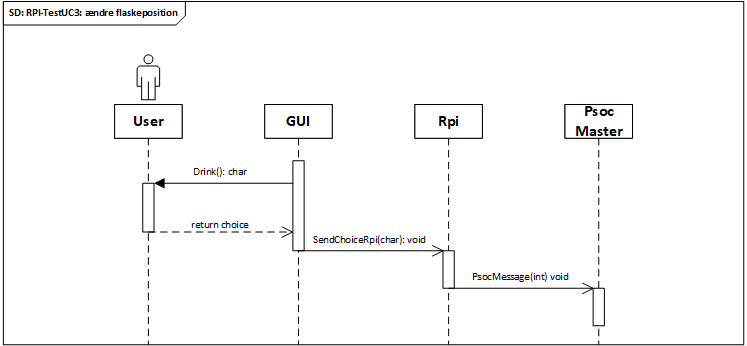
\includegraphics[width=1\textwidth]{Images/Applikationsmodeller/rpi/rpi_sekvensdiagramTestUC3.png}
    \caption{Sekvensdiagram for Rpi i TUC3}
    \label{fig:sdTUC3Rpi}
\end{figure}

\begin{figure}[H]
    \centering
    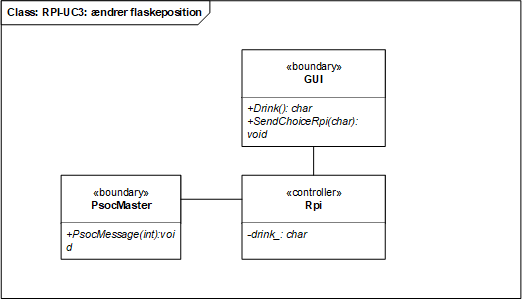
\includegraphics[width=1\textwidth]{Images/Applikationsmodeller/rpi/rpi_UdvidetklassediagramTestUC3.png}
    \caption{Udvidet klassediagram for Rpi i TUC3}
    \label{fig:UcdTUC3Rpi}
\end{figure}

\subsubsection{TUC4}

\begin{figure}[H]
    \centering
    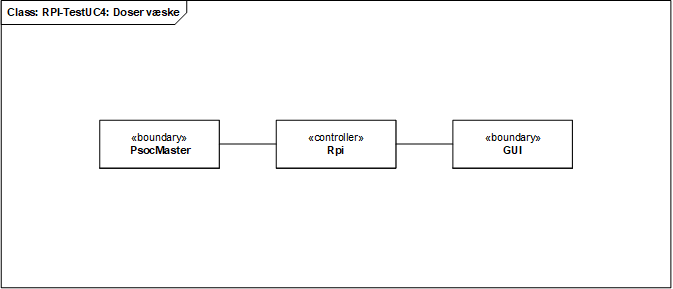
\includegraphics[width=1\textwidth]{Images/Applikationsmodeller/rpi/rpi_klassediagramTestUC4.png}
    \caption{Indledende klassediagram for Rpi i TUC4}
    \label{fig:cdTUC4Rpi}
\end{figure}

\begin{figure}[H]
    \centering
    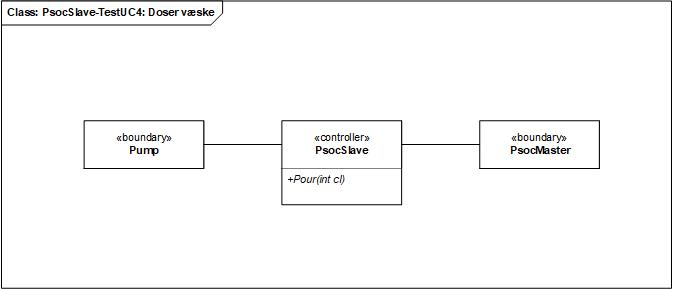
\includegraphics[width=1\textwidth]{Images/PsocSlaveTUC4.jpg}
    \caption{Indledende klassediagram for Psoc slave i TUC4}
    \label{fig:cdTUC4Rpi}
\end{figure}


\begin{figure}[H]
    \centering
    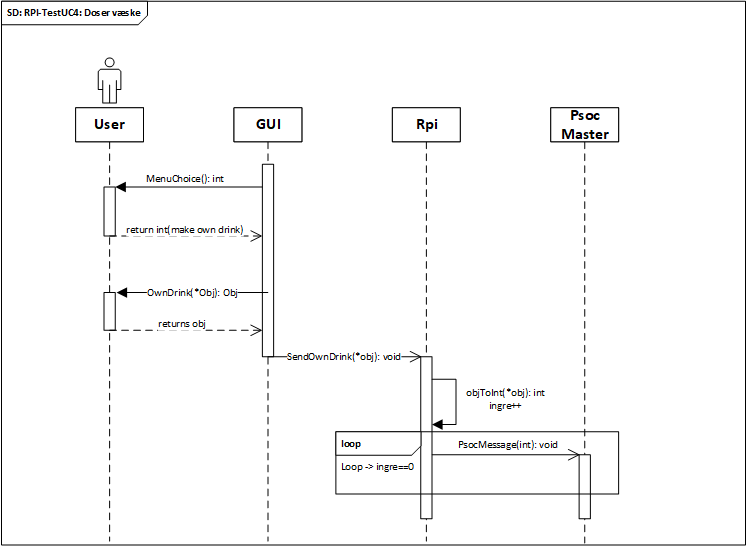
\includegraphics[width=1\textwidth]{Images/Applikationsmodeller/rpi/rpi_sekvensdiagramTestUC4.png}
    \caption{Sekvensdiagram for Rpi i TUC4}
    \label{fig:sdTUC4Rpi}
\end{figure}

\begin{figure}[H]
    \centering
    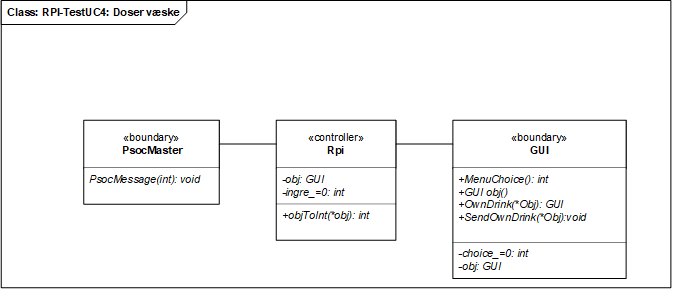
\includegraphics[width=1\textwidth]{Images/Applikationsmodeller/rpi/rpi_UdvidetklassediagramTestUC4.png}
    \caption{Udvidet klassediagram for Rpi i TUC4}
    \label{fig:UcdTUC4Rpi}
\end{figure}

\subsubsection{TUC5}

\begin{figure}[H]
    \centering
    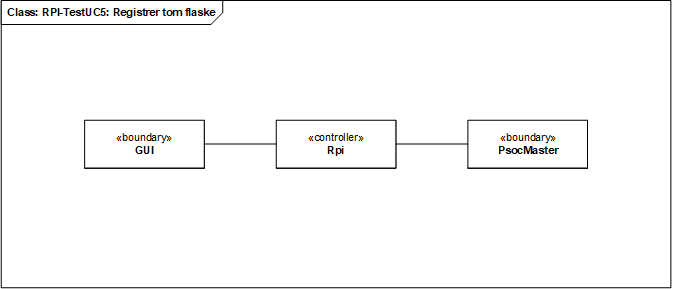
\includegraphics[width=1\textwidth]{Images/Applikationsmodeller/rpi/rpi_klassediagramTestUC5.png}
    \caption{Indledende klassediagram for Rpi i TUC5}
    \label{fig:cdTUC5Rpi}
\end{figure}

\begin{figure}[H]
    \centering
    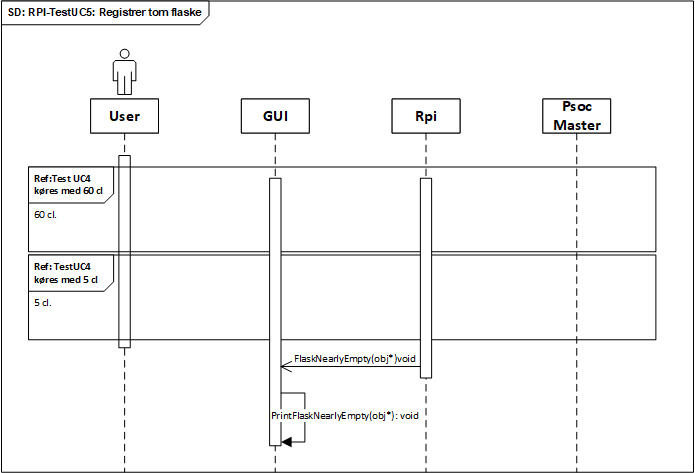
\includegraphics[width=1\textwidth]{Images/Applikationsmodeller/rpi/rpi_sekvensdiagramTestUC5.png}
    \caption{Sekvensdiagram for Rpi i TUC5}
    \label{fig:sdTUC5Rpi}
\end{figure}

\begin{figure}[H]
    \centering
    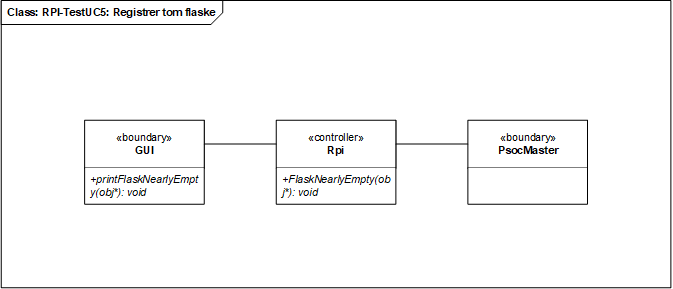
\includegraphics[width=1\textwidth]{Images/Applikationsmodeller/rpi/rpi_UdvidetklassediagramTestUC5.png}
    \caption{Udvidet klassediagram for Rpi i TUC5}
    \label{fig:UcdTUC5Rpi}
\end{figure}

\subsubsection{TUC6}

\begin{figure}[H]
    \centering
    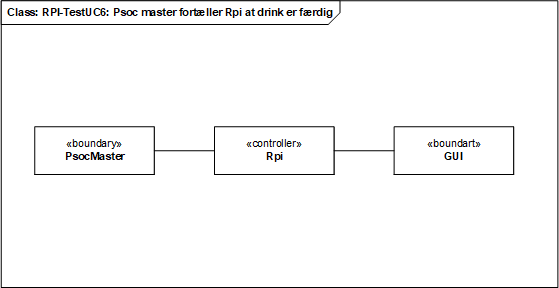
\includegraphics[width=1\textwidth]{Images/Applikationsmodeller/rpi/rpi_klassediagramTestUC6.png}
    \caption{Indledende klassediagram for Rpi i TUC6}
    \label{fig:cdTUC6Rpi}
\end{figure}

\begin{figure}[H]
    \centering
    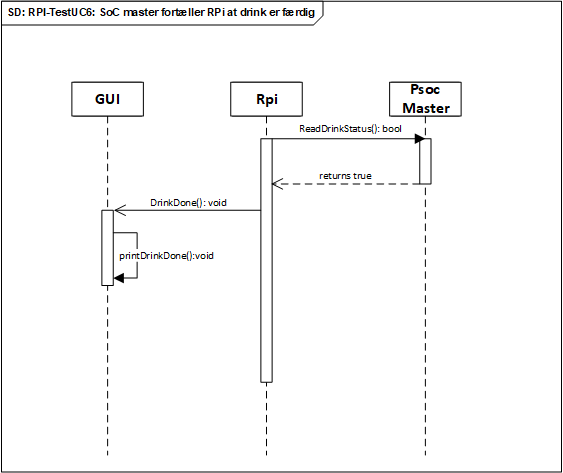
\includegraphics[width=1\textwidth]{Images/Applikationsmodeller/rpi/rpi_sekvensdiagramTestUC6.png}
    \caption{Sekvensdiagram for Rpi i TUC6}
    \label{fig:sdTUC6Rpi}
\end{figure}

\begin{figure}[H]
    \centering
    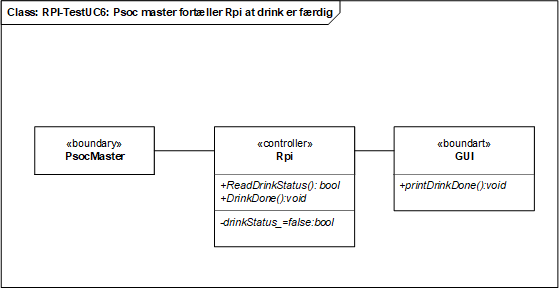
\includegraphics[width=1\textwidth]{Images/Applikationsmodeller/rpi/rpi_UdvidetklassediagramTestUC6.png}
    \caption{Udvidet klassediagram for Rpi i TUC6}
    \label{fig:UcdTUC6Rpi}
\end{figure}

\subsubsection{Samlet klassediagram for Rpi}

\begin{figure}[H]
    \centering
    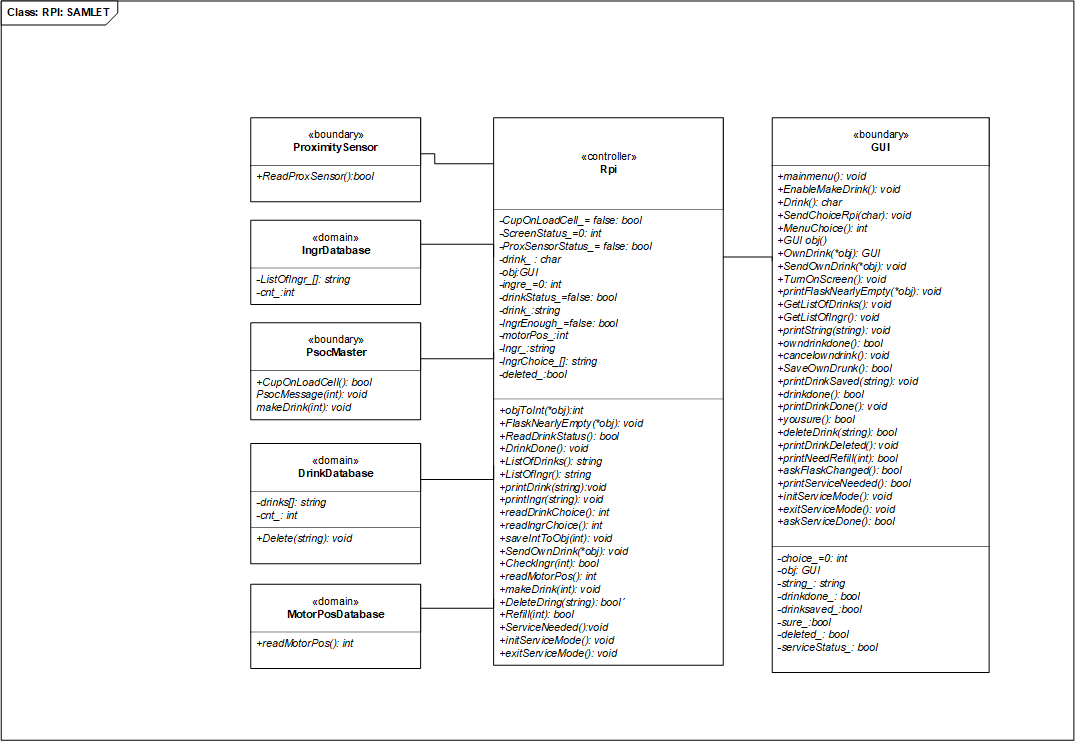
\includegraphics[width=1\textwidth]{Images/Applikationsmodeller/rpi/Samlet_klassediagram.png}
    \caption{Samlet klassediagram for Rpi}
    \label{fig:Samlet - Rpi}
\end{figure}

\subsection{Applikationsmodel for PSoC Master}
\subsubsection{UC1}

\begin{figure}[H]
	\centering
	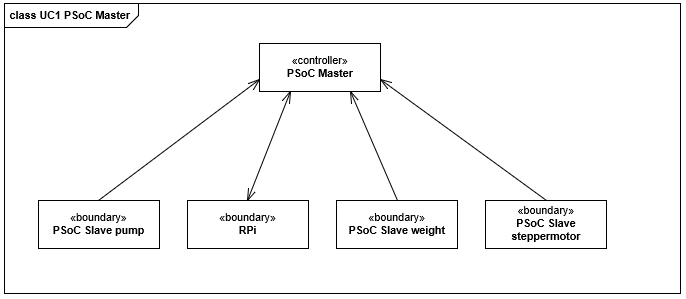
\includegraphics[width=1\textwidth]{Images/Applikationsmodeller/PSoCMaster/UC1_cd_PSoC_Master.png}
	\caption{Indledende klassediagram for PSoC Master UC1}
	\label{fig:cdUC1PSoCMaster}
\end{figure}

\begin{figure}[H]
	\centering
	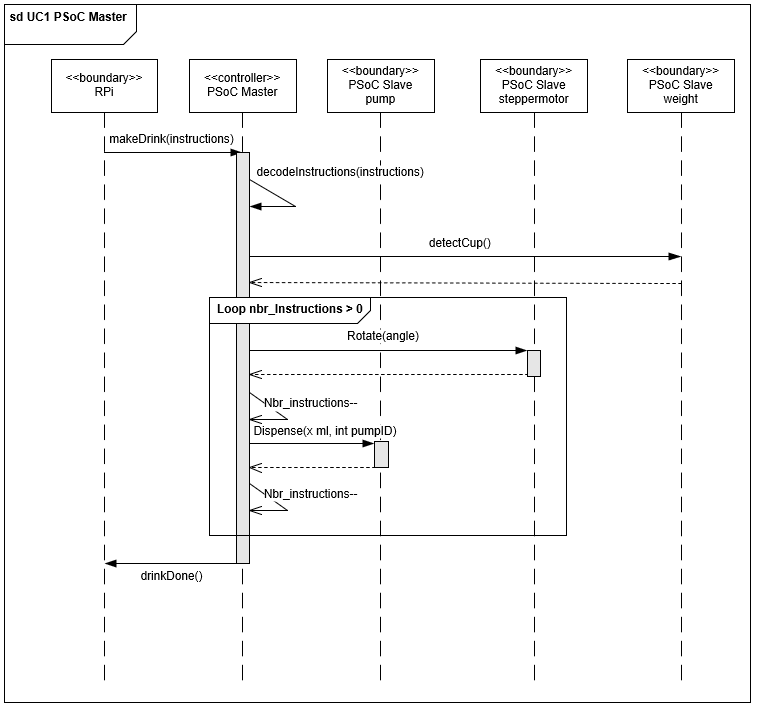
\includegraphics[width=1\textwidth]{Images/Applikationsmodeller/PSoCMaster/UC1_sd_PSoC_Master.png}
	\caption{Sekvensdiagram for UC1 PSoC Master}
	\label{fig:sdUC1PSoCMaster}
\end{figure}

\begin{figure}[H]
	\centering
	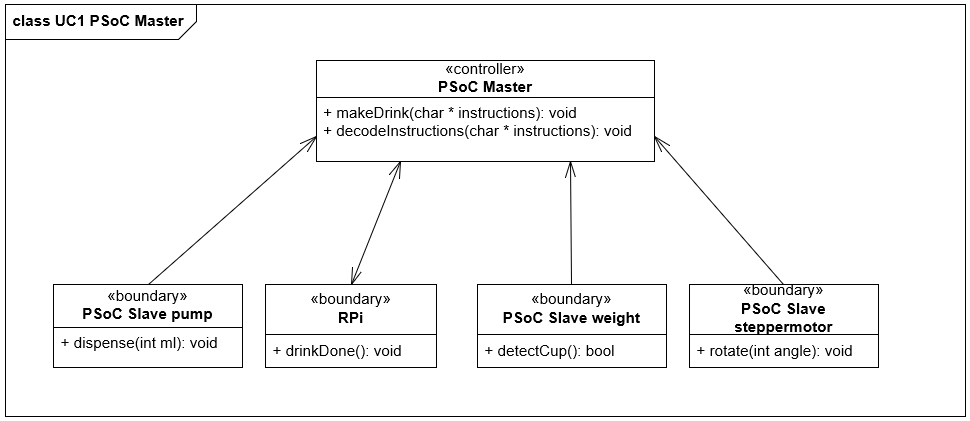
\includegraphics[width=1\textwidth]{Images/Applikationsmodeller/PSoCMaster/UC1_cd_PSoC_Master_final.png}
	\caption{Færdigt klassediagram for UC1 PSoC Master}
	\label{fig:cdUC1PSoCMaster_final}
\end{figure}

\subsubsection{TUC2}

\begin{figure}[H]
	\centering
	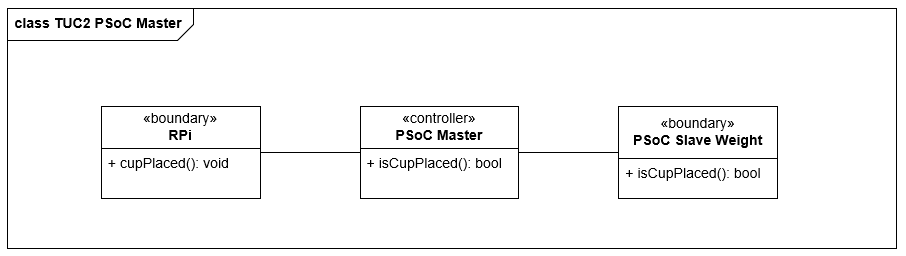
\includegraphics[width=1\textwidth]{Images/Applikationsmodeller/PSoCMaster/TUC2_cd_PSoC_Master.png}
	\caption{Klassediagram for TUC2 PSoC Master}
	\label{fig:cdTUC2PSoCMaster}
\end{figure}

\begin{figure}[H]
	\centering
	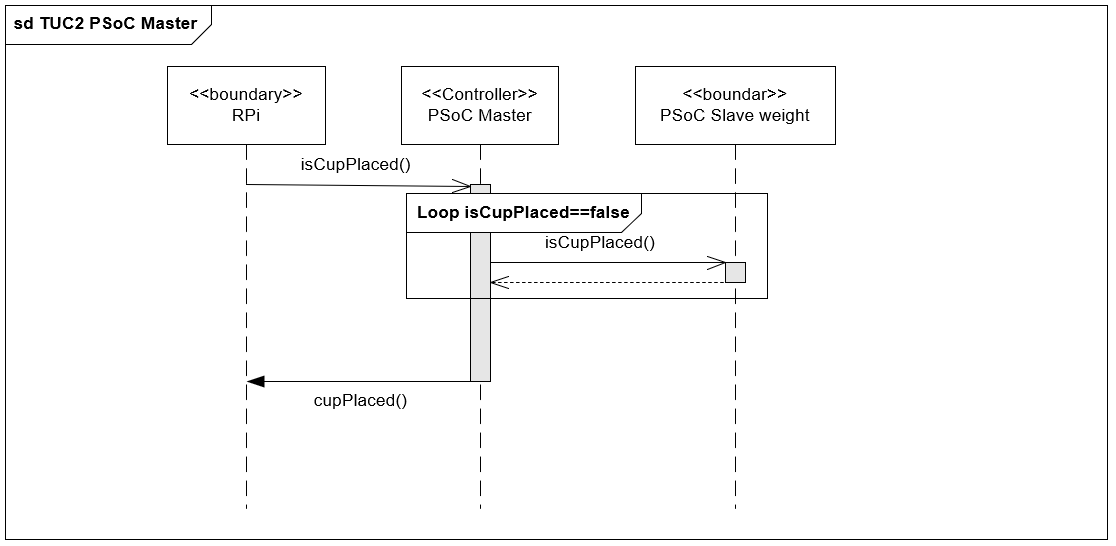
\includegraphics[width=1\textwidth]{Images/Applikationsmodeller/PSoCMaster/TUC2_sd_PSoC_Master.png}
	\caption{Sekvendiagram for TUC2 PSoC Master}
	\label{fig:sdTUC2PSoCMaster}
\end{figure}

\begin{figure}[H]
	\centering
	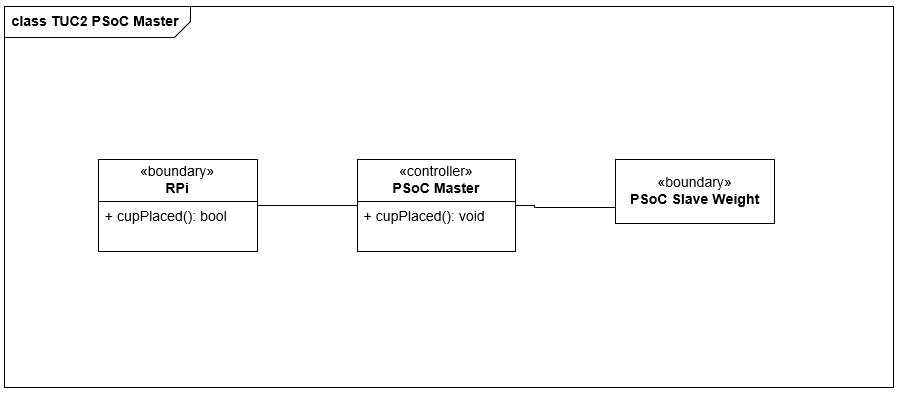
\includegraphics[width=1\textwidth]{Images/Applikationsmodeller/PSoCMaster/TUC2_cd_PSoC_Master_final.png}
	\caption{Færdigt klassediagram for TUC2 PSoC Master}
	\label{fig:cdTUC2PSoCMaster_final}
\end{figure}

\subsubsection{TUC3}
\begin{figure}[H]
	\centering
	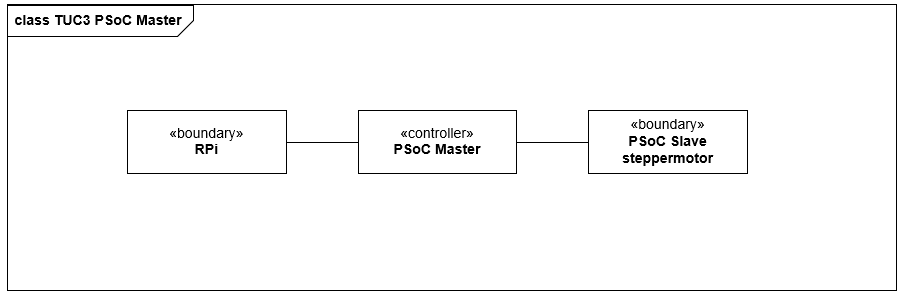
\includegraphics[width=1\textwidth]{Images/Applikationsmodeller/PSoCMaster/TUC3_cd_PSoC_Master.png}
	\caption{Klassediagram for TUC3 PSoC Master}
	\label{fig:cdTUC3PSoCMaster}
\end{figure}

\begin{figure}[H]
	\centering
	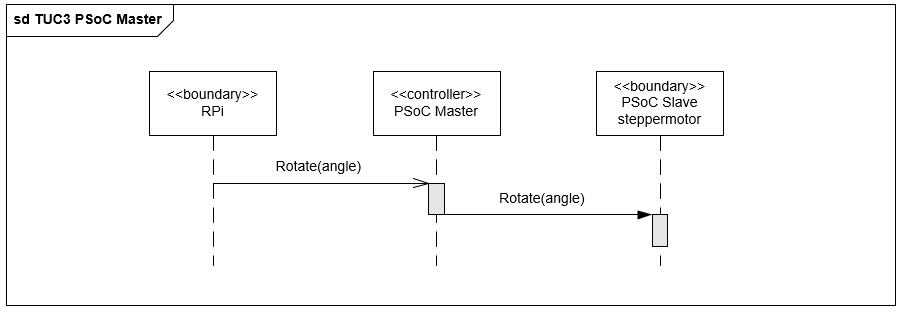
\includegraphics[width=1\textwidth]{Images/Applikationsmodeller/PSoCMaster/TUC3_sd_PSoC_Master.png}
	\caption{Sekvensdiagram for TUC3 PSoC Master}
	\label{fig:sdTUC3PSoCMaster}
\end{figure}

\begin{figure}[H]
	\centering
	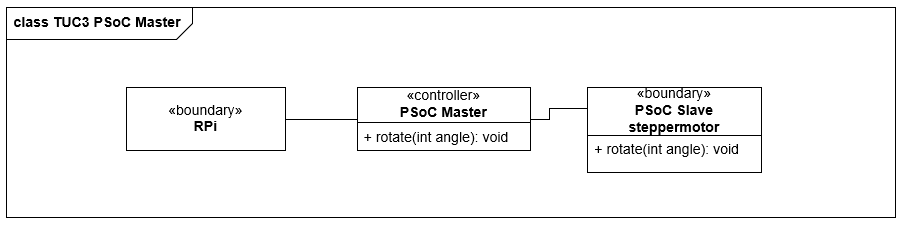
\includegraphics[width=1\textwidth]{Images/Applikationsmodeller/PSoCMaster/TUC3_cd_PSoC_Master_final.png}
	\caption{Færdigt klassediagram for TUC3 PSoC Master}
	\label{fig:cdTUC3PSoCMaster_final}
\end{figure}
\subsubsection{TUC4}
\begin{figure}[H]
	\centering
	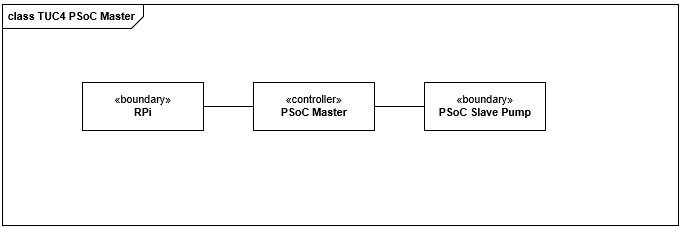
\includegraphics[width=1\textwidth]{Images/Applikationsmodeller/PSoCMaster/TUC4_cd_PSoC_Master.png}
	\caption{Klassediagram for TUC4 PSoC Master}
	\label{fig:cdTUC4PSoCMaster}
\end{figure}

\begin{figure}[H]
	\centering
	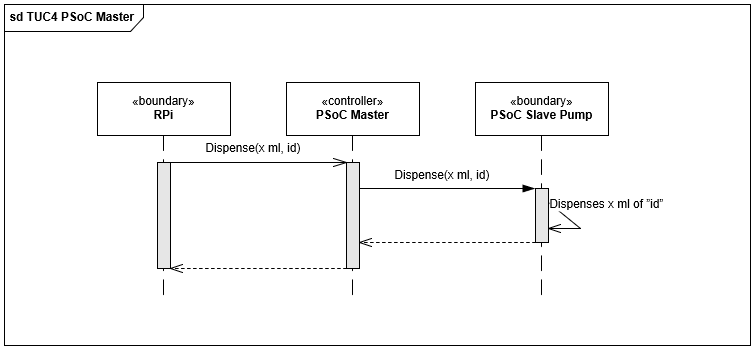
\includegraphics[width=1\textwidth]{Images/Applikationsmodeller/PSoCMaster/TUC4_sd_PSoC_Master.png}
	\caption{Sekvensdiagram for TUC4 PSoC Master}
	\label{fig:sdTUC3PSoCMaster}
\end{figure}
\begin{figure}[H]
	\centering
	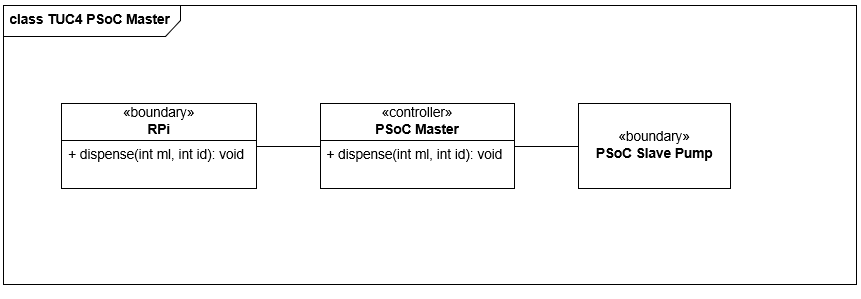
\includegraphics[width=1\textwidth]{Images/Applikationsmodeller/PSoCMaster/TUC4_cd_PSoC_Master_final.png}
	\caption{Færdigt klassediagram for TUC4 PSoC Master}
	\label{fig:cdTUC4PSoCMaster_final}
\end{figure}

\subsubsection{TUC6 - PSoC Master fortæller RPi at drink er færdig}
\begin{figure}[H]
	\centering
	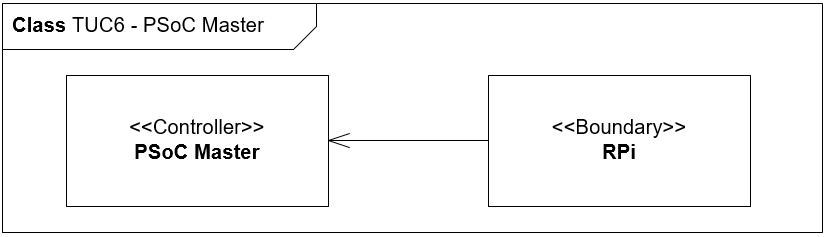
\includegraphics[width=1\textwidth]{Images/Applikationsmodeller/PSoCMaster/class1.png}
	\caption{Første klassediagram for TUC6 for PSoC Master}
	\label{fig:cdTUC6PSoCMaster_first}
\end{figure}

\begin{figure}[H]
	\centering
	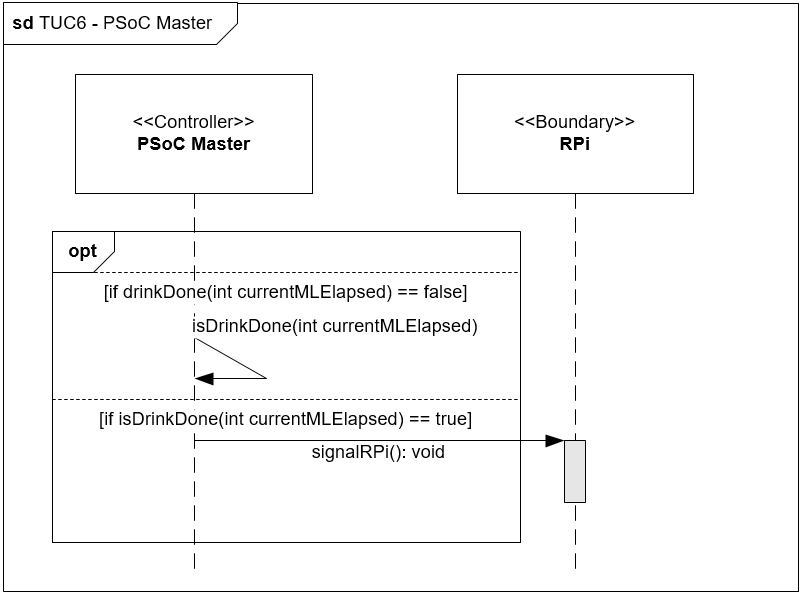
\includegraphics[width=1\textwidth]{Images/Applikationsmodeller/PSoCMaster/PSoCMasterTUC6_Sekvensdiagram.png}
	\caption{Sekvensdiagram for TUC6 PSoC Master}
	\label{fig:sdTUC6PSoCMaster}
\end{figure}

\begin{figure}[H]
	\centering
	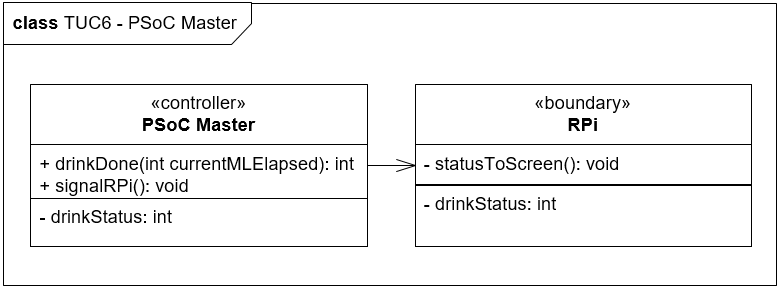
\includegraphics[width=1\textwidth]{Images/Applikationsmodeller/PSoCMaster/PSoCMasterTUC6_Udv_class.png}
	\caption{Færdigt klassediagram for TUC6 -  PSoC Master}
	\label{fig:cdTUC6PSoCMaster_final}
\end{figure}

\subsection{Applikationsmodel for PSoC Slaven - Vægtsensor}

\subsubsection{UC1}
\begin{figure}[H]
	\centering
	\includegraphics[width=1\textwidth]{Images/Applikationsmodeller/PSoCWeight/classAppWeightUC1.png}
	\caption{Klassediagram for "PSoC slave weight" UC1}
	\label{fig:classAppWeightUC1}
\end{figure}

\begin{figure}[H]
	\centering
	\includegraphics[width=1\textwidth]{Images/Applikationsmodeller/PSoCWeight/sdAppWeightUC1.png}
	\caption{Sekvensdiagram for "PSoC slave weight" UC1}
	\label{fig:sdAppWeightUC1}
\end{figure}

\begin{figure}[H]
	\centering
	\includegraphics[width=1\textwidth]{Images/Applikationsmodeller/PSoCWeight/ClassExtAppWeightUC1.png}
	\caption{Udvidet klassediagram for "PSoC slave weight" UC1}
	\label{fig:ClassExtAppWeightUC1}
\end{figure}

\subsubsection{TUC2}
\begin{figure}[H]
	\centering
	\includegraphics[width=1\textwidth]{Images/Applikationsmodeller/PSoCWeight/Class_TUC2_PSoC_Slave_Weight.png}
	\caption{Klassediagram for "PSoC slave weight" TUC2}
	\label{fig:cdTUC2PSoCSlaveWeight}
\end{figure}

%\subsubsection{TUC2}
\begin{figure}[H]
	\centering
	\includegraphics[width=1\textwidth]{Images/Applikationsmodeller/PSoCWeight/Sd_TUC2_PSoC_Slave_Weight_Temporary_Crop.png}
	\caption{Sekvensdiagram "PSoC slave weight" TUC2}
	\label{fig:sdTUC2PSoCSlaveWeight}
\end{figure}

%\subsubsection{TUC2}
\begin{figure}[H]
	\centering
	\includegraphics[width=1\textwidth]{Images/Applikationsmodeller/PSoCWeight/Class_TUC2_PSoC_Slave_Weight.png}
	\caption{Klassediagram for "PSoC slave weight" TUC2}
	\label{fig:classTUC2PSoCSlaveWeight}
\end{figure}

\subsection{Applikationsmodel for PSoC Slaven - Pumpestyring}
\subsubsection{UC1}
\begin{figure}[H]
	\centering
	\includegraphics[width=1\textwidth]{Images/Applikationsmodeller/UC1_cd_PSoC_Slave_pump.png}
	\caption{Klassediagram for "PSoC slave pump" UC1}
	\label{fig:cdUC1PSoCSlavePump}
\end{figure}

\begin{figure}[H]
	\centering
	\includegraphics[width=1\textwidth]{Images/Applikationsmodeller/UC1_sd_PSoC_Slave_pump.png}
	\caption{Sekvensdiagram for PSoC Slave Pump UC1}
	\label{fig:sdUC1PSoCSlavePump}
\end{figure}

\begin{figure}[H]
	\centering
	\includegraphics[width=1\textwidth]{Images/Applikationsmodeller/UC1_cd_PSoC_Slave_pump_final.png}
	\caption{Færdigt klassediagram for UC1 PSoC Slave Pump}
	\label{fig:cdUC1PSoCSlavePump_final}
\end{figure}


\subsection{Applikationsmodel for PSoC Slaven - Steppermotor}
\subsubsection{UC1}
\begin{figure}[H]
	\centering
	\includegraphics[width=1\textwidth]{Images/Applikationsmodeller/PSoCStepper/ClassSteppermotorUC1.png}
	\caption{Indledende klassediagram for PSoC Slave - Steppermotor UC1}
	\label{fig:preClassStepperUC1}
\end{figure}

\begin{figure}[H]
	\centering
	\includegraphics[width=1\textwidth]{Images/Applikationsmodeller/PSoCStepper/sdSteppermotorUC1.png}
	\caption{Sekvensdiagram for PSoC Slave - Steppermotor UC1}
	\label{fig:sdStepperUC1}
\end{figure}

\begin{figure}[H]
	\centering
	\includegraphics[width=1\textwidth]{Images/Applikationsmodeller/PSoCStepper/ClassextSteppermotorUC1.png}
	\caption{Udvidet klassediagram for PSoC Slave - Steppermotor UC1}
	\label{fig:postClassStepperUC1}
\end{figure}

\subsubsection{TUC3}
\begin{figure}[H]
	\centering
	\includegraphics[width=1\textwidth]{Images/Applikationsmodeller/PSoCStepper/first_class_TUC_3_PSoC_Slave_steppermotor.png}
	\caption{Klassediagram for PSoC Slave - Steppermotor TUC3}
	\label{fig:preClassStepperTUC3}
\end{figure}

\begin{figure}[H]
	\centering
	\includegraphics[width=1\textwidth]{Images/Applikationsmodeller/PSoCStepper/sd_TUC_3_PSoC_Slave_steppermotor.png}
	\caption{Sekvensdiagram for PSoC Slave - Steppermotor TUC3}
	\label{fig:sdStepperTUC3}
\end{figure}

\begin{figure}[H]
	\centering
	\includegraphics[width=1\textwidth]{Images/Applikationsmodeller/PSoCStepper/second_class_TUC_3_PSoC_Slave_steppermotor.png}
	\caption{Udvidet klassediagram for PSoC Slave - Steppermotor TUC3}
	\label{fig:postClassStepperTUC3}
\end{figure}